\documentclass{beamer}
%\usepackage[margin=1in]{geometry}
\usepackage{amsthm,amsmath,amsfonts,hyperref,graphicx,color,multicol}
\usepackage{enumitem,tikz}

%%%%%%%%%%
%Beamer Template Customization
%%%%%%%%%%
\setbeamertemplate{navigation symbols}{}
\setbeamertemplate{theorems}[ams style]
\setbeamertemplate{blocks}[rounded]

\definecolor{Blu}{RGB}{43,62,133} % UWEC Blue
\setbeamercolor{structure}{fg=Blu} % Titles

%Unnumbered footnotes:
\newcommand{\blfootnote}[1]{%
	\begingroup
	\renewcommand\thefootnote{}\footnote{#1}%
	\addtocounter{footnote}{-1}%
	\endgroup
}


%%%%%%%%%%
%Custom Commands
%%%%%%%%%%
\newcommand{\R}{\mathbb{R}}
\newcommand{\veca}{\vec{a}}
\newcommand{\vecb}{\vec{b}}
\newcommand{\vece}{\vec{e}}
\newcommand{\vecu}{\vec{u}}
\newcommand{\vecv}{\vec{v}}
\newcommand{\vecw}{\vec{w}}
\newcommand{\vecx}{\vec{x}}
\newcommand{\zerovector}{\vec{0}}

\newcommand{\ds}{\displaystyle}

\newcommand{\fn}{\insertframenumber}

\newcommand{\rank}{\operatorname{rank}}
\newcommand{\adj}{\operatorname{adj}}

\newcommand{\blank}[1]{\underline{\hspace*{#1}}}


%%%%%%%%%%
%Custom Theorem Environments
%%%%%%%%%%
\theoremstyle{definition}
\newtheorem{exercise}{Exercise}
\newtheorem{question}[exercise]{Question}
\newtheorem*{defn}{Definition}
\newtheorem*{exa}{Example}
\newtheorem*{disc}{Group Discussion}
\newtheorem*{nb}{Note}
\newtheorem*{recall}{Recall}
\renewcommand{\emph}[1]{{\color{blue}\texttt{#1}}}

\definecolor{Gold}{RGB}{237, 172, 26}
%Statement block
\newenvironment{statementblock}[1]{%
	\setbeamercolor{block body}{bg=Gold!20}
	\setbeamercolor{block title}{bg=Gold}
	\begin{block}{\textbf{#1.}}}{\end{block}}





\begin{document}
	\title{Math 324: Linear Algebra}
	\subtitle{Section 4.5: Basis}
	\author{Mckenzie West}
	\date{Last Updated: \today}
\begin{frame}
\maketitle
\end{frame}

\begin{frame}{\insertframenumber}
	\begin{block}{\textbf{Last Time.}}
	\begin{itemize}[label=--]
		\item Linear Independence
	\end{itemize}
	\end{block}
	\begin{block}{\textbf{Today.}}
		\begin{itemize}[label=--]
			\item Basis
		\end{itemize}
	\end{block}
\end{frame}

\begin{frame}{\fn}
	\begin{defn}
		A set of vectors $S=\{\vec v_1,\vec v_2,\dots,\vec v_n\}$ in a vector space $V$ is called a \emph{basis} for $V$ if both (\textbf{1}) $S$ spans $V$ and (\textbf{2}) $S$ is linearly independent.
	\end{defn}
	\begin{nb}
		Bases (base-eaze) are ``Goldilocks sets'' in that they aren't too small (\textbf{1}) and they aren't too big (\textbf{2}).
		
		Recall that for out usual vector spaces, using the vectors as columns of a matrix,
		\begin{center}
			\begin{tabular}{rcl} 
				spanning &$\longleftrightarrow$& no zero rows in RREF\\
				linearly independent &$\longleftrightarrow$& no free variables
			\end{tabular}
		\end{center}
	\end{nb}
\end{frame}
\begin{frame}{\fn}
	\begin{exercise}
		Explain why $S=\{(1,0,0),(0,1,0),(0,0,1)\}$ is a basis for $\R^3$. 
	\end{exercise}
	\begin{defn}
		The basis $S=\{(1,0,0),(0,1,0),(0,0,1)\}$ is called the \emph{standard basis for $\R^3$}.  The \emph{standard basis for $\R^n$} is the set $S=\{\vec e_1,\vec e_2,\dots,\vec e_n\}$ of vectors where,
		$$\begin{array}{rcl}
		\vec e_1&=&(1,0,\dots,0)\\
		\vec e_2 &=&(0,1,\dots,0)\\
		&\vdots\\
		\vec e_n&=&(0,0,\dots,1).
		\end{array}$$
	\end{defn}
\end{frame}
\begin{frame}{\fn}
	\begin{exercise}\label{exercise:basisforR2}
		Show that $S=\{(1,2),(5,-2)\}$ is a basis for $\R^2$. That is, show that $S$ is linearly independent and spans $\R^2$.
	\end{exercise}
	\begin{exercise}
		Which of the following are bases for $\R^3$? Explain why or why not.
		\begin{enumerate}[label=(\alph*)]
			\item $\{(1,0,1),(1,1,0),(0,1,1),(1,1,1)\}$
			\item $\{(4,0,2),(1,1,3)\}$
			\item $\{(1,1,1),(1,1,0),(1,0,0)\}$
			\item $\{(1,2,3),(4,5,6),(7,8,9)\}$
		\end{enumerate}
	\end{exercise}
\end{frame}
\begin{frame}{\fn}
	\begin{exercise}
		Explain why $S=\{1,x,x^2,x^3\}$ is a basis for $P_3$, called the \emph{standard basis for $P_3$}.
	\end{exercise}
	\begin{exa}
		The \emph{standard basis for $M_{2,2}$} is the set 
		\[S=\left\{\begin{bmatrix}1&0\\0&0\end{bmatrix},\begin{bmatrix}0&1\\0&0\end{bmatrix},\begin{bmatrix}0&0\\1&0\end{bmatrix},\begin{bmatrix}0&0\\0&1\end{bmatrix}\right\}.\]
	\end{exa}
	\begin{exercise}
		What do you think the standard basis for $M_{m,n}$ is?
	\end{exercise}
\end{frame}
\begin{frame}{\fn}
	\begin{defn}
		If a basis exists for a vector space, we call it \emph{finite dimensional} otherwise a vector space is said to be \emph{infinite dimensional}.
	\end{defn}
	\begin{exa}
		The vector space $P$ of all polynomials is infinite dimensional, as is $C(-\infty,\infty)$ the collection of all real valued continuous functions.
	\end{exa}
\end{frame}
\begin{frame}{\fn}
	\begin{block}{\textbf{Brain Break.}}
		What’s your current favorite show to binge watch?
		\begin{center}
			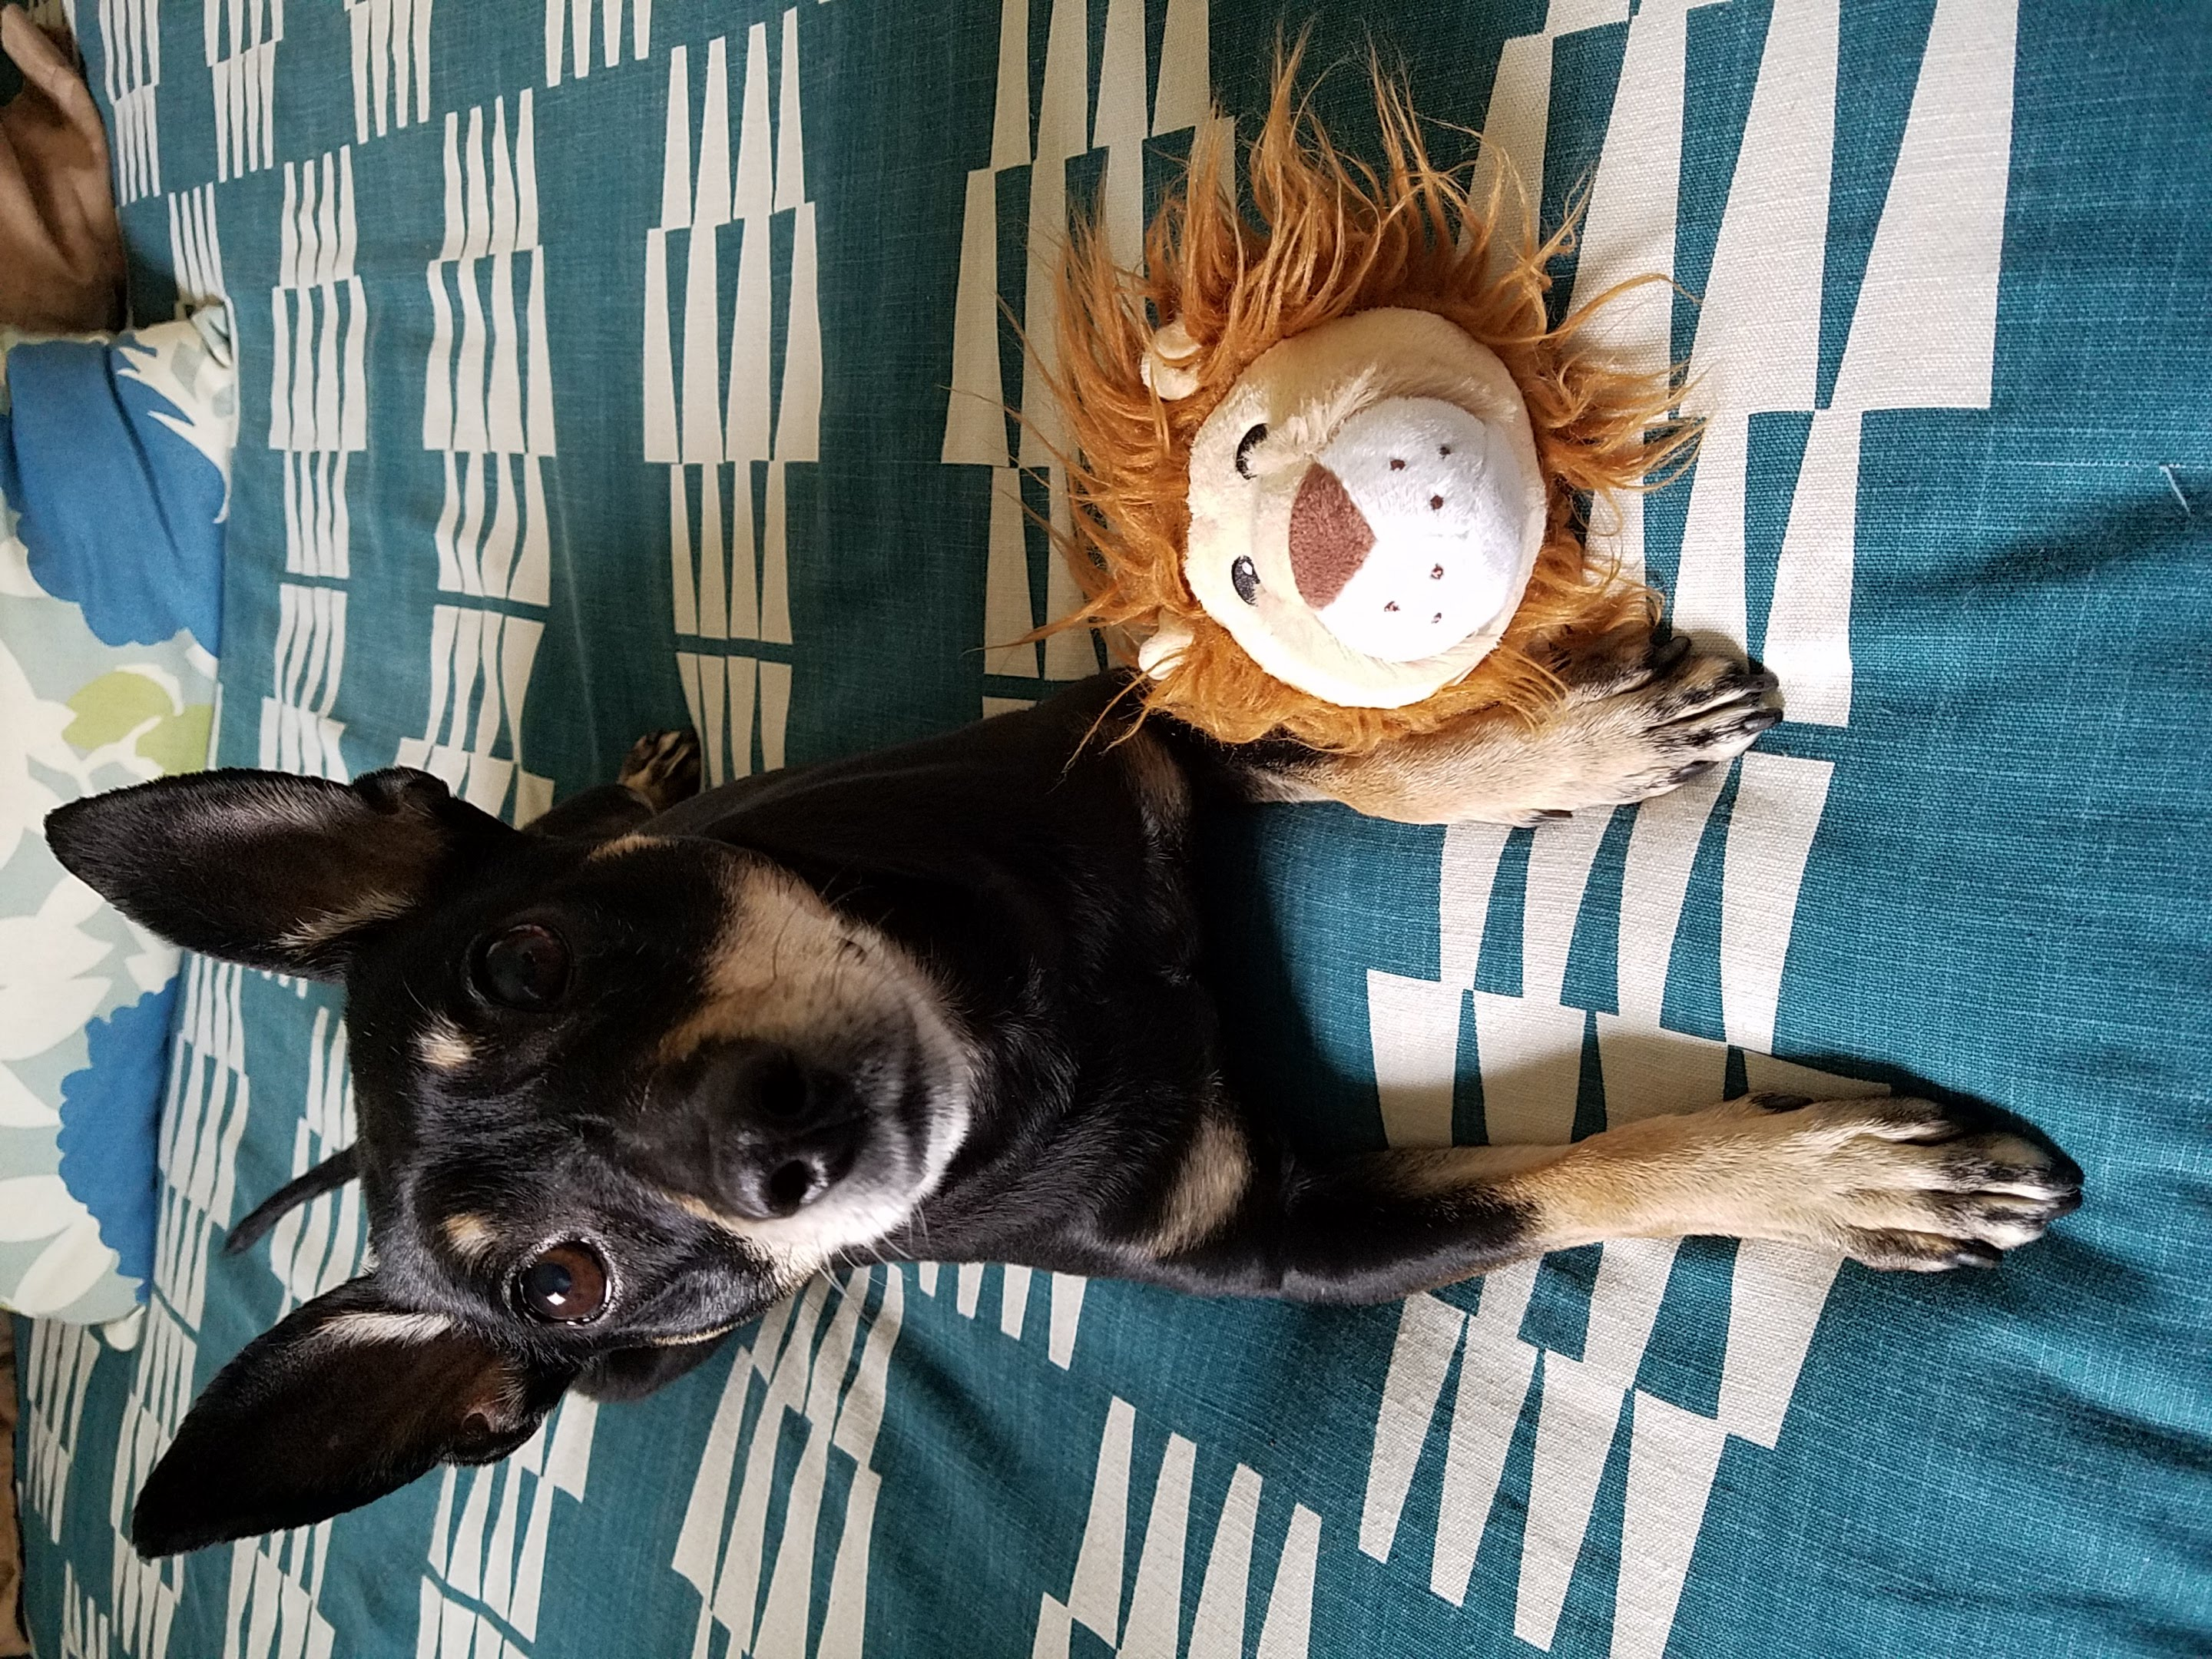
\includegraphics[angle=270,width=1.5in]{../images/lion_Pepper}
			\vskip .15in
			\footnotesize
			Turns out Pepper doesn't have any tiger toys, so we're settling for Lion King.
		\end{center}
	\end{block}
\end{frame}
\begin{frame}{\fn}
	\begin{statementblock}{Theorem 4.9}
		If $S=\{\vec v_1,\vec v_2,\dots, \vec v_n\}$ is a basis for a vector space $V$, then every vector in $V$ can be written in one and only one way as a linear combination of the vectors in $S$.
	\end{statementblock}
	\begin{nb}
		The proof of this theorem is in the book.  It uses the fact that since $S$ is a basis, its elements are linearly independent and so there is only 1 way to represent the zero vector.
	\end{nb}
\end{frame}
\begin{frame}{\fn}
	\begin{exa}
		Every vector $\vec u=(x,y)$ in $\R^2$ can be written uniquely in terms of the vectors in the basis $S=\{(1,2),(5,-2)\}$ from exercise~\ref{exercise:basisforR2}.  How might you show there is a unique solution to \[c_1(1,2)+c_2(5,-2)=(x,y),\]
		no matter the value of $x$ and $y$?
		
		I suggest writing down the matrix $A$ so that $A\begin{bmatrix}c_1\\c_2\end{bmatrix}=\begin{bmatrix}x\\y\end{bmatrix}$.
	\end{exa}
\end{frame}
\begin{frame}{\fn}
	\begin{statementblock}{Theorem 4.10}
		If $S=\{\vec v_1,\vec v_2,\dots,\vec v_n\}$ is a basis for a vector space $V$, then every set containing more than $n$ vectors in $V$ is linearly dependent.
	\end{statementblock}
	\begin{nb}
		The proof of Theorem 4.10 is available in the book.  It relies on the fact that you can write the vectors in the set $\{\vec u_1,\vec u_2,\dots,\vec u_m\}$ $(m>n)$ in terms of the vectors in the basis $S$ and insert them into the equation $k_1\vec u_1+k_2\vec u_2+\cdots+k_m\vec u_m=\vec 0$.  Ultimately you will get a homogeneous system with more variable then equations, so there is a nontrivial solution.
	\end{nb}
\end{frame}
\begin{frame}{\fn}
	\begin{exercise}
		Explain by looking, no computations only references to theorems, why the following are linearly dependent:
		\begin{enumerate}[label=(\alph*)]
			\item $S=\{(1,1,0),(1,0,1),(0,1,1),(1,1,1)\}$ in $\R^3$
			\item $S=\{x-1,x+1,x^2-1,x^2+1\}$ in $P_2$
			\item $S=\{(6,2),(18,6)\}$ in $\R^2$
			\item $S=\left\{\begin{bmatrix}1&2\\3&4\end{bmatrix},\begin{bmatrix}2&1\\3&4\end{bmatrix},\begin{bmatrix}1&2\\4&3\end{bmatrix},\begin{bmatrix}2&1\\4&3\end{bmatrix},\begin{bmatrix}3&4\\1&2\end{bmatrix}\right\}$.
		\end{enumerate}
	\end{exercise}
\end{frame}
\end{document}

